% Created 2024-05-23 Thu 22:39
% Intended LaTeX compiler: pdflatex
\documentclass[presentation]{beamer}
\usepackage{luatexja}

                 \usepackage{luatexja}
                 \usepackage{luatexja-preset}
\usetheme{Madrid}
\usecolortheme{beetle}
\author{Atsushi Odagiri}
\date{2024-04-25}
\title{パッケージを配ろう}
\hypersetup{
 pdfauthor={Atsushi Odagiri},
 pdftitle={パッケージを配ろう},
 pdfkeywords={},
 pdfsubject={},
 pdfcreator={Emacs 29.3 (Org mode 9.6.15)}, 
 pdflang={English}}
\begin{document}

\maketitle
\begin{frame}{Outline}
\tableofcontents
\end{frame}

\section{パッケージを配ろう}
\label{sec:org2dad1c8}
\begin{frame}[label={sec:org7697459}]{お前誰よ}
\begin{block}{}
\begin{itemize}
\item Atsushi Odagiri
\item Open Collector
\item Pythonは1.5くらいのころから
\end{itemize}
\end{block}

\begin{block}{}
\begin{center}

\includegraphics[width=2cm]{./r-penta512.png}
\end{center}

\begin{center}

\includegraphics[width=2cm]{./oc-logo.png}
\end{center}
\begin{center}

\includegraphics[width=2cm]{./logo-w.png}
\end{center}
\end{block}
\end{frame}
\section{パッケージを配るということ}
\label{sec:orgdcc8106}
\begin{frame}[label={sec:orge5b02c1}]{パッケージエコシステム}
\begin{itemize}
\item 作る
\item 配る
\item 使う
\end{itemize}
\end{frame}

\begin{frame}[label={sec:org970e5ac}]{パッケージを配るということ}
\begin{itemize}
\item 広く一般に向けて配る
\item 狭い範囲で限られた利用のために配る
\end{itemize}
\end{frame}

\begin{frame}[label={sec:org168d7d0},fragile]{広く一般に向けてpypiで配る}
 \begin{itemize}
\item PyPAツールのデフォルト
\item \texttt{tween} でアップロード
\item \texttt{pip} がダウンロードしてインストール
\end{itemize}
\end{frame}

\begin{frame}[label={sec:org9a6fe1f}]{狭い範囲で限られた利用のために配る}
\begin{itemize}
\item マイクロサービスのそれぞれて使うようなライブラリ
\item 特殊なパッチをあてたローカルフレーバーライブラリ
\end{itemize}
\end{frame}

\begin{frame}[label={sec:org212a02d}]{狭い範囲で配る}
\begin{itemize}
\item 社内ネットワークやVPNの中で
\item k8sやvpcの中で
\item 範囲内のIPアドレスにだけ
\item 認証をつけたい
\end{itemize}
\end{frame}

\begin{frame}[label={sec:org3d9af59},fragile]{httplib.server でのお手軽repository}
 \begin{itemize}
\item ダウンロードできるリンクがあればいいので \texttt{http} モジュールでサーバーを起動するだけ
\item wheelファイルのあるディレクトリで実行
\end{itemize}

\begin{verbatim}
python3 -m pip download pyramid
python3 -m http.server
\end{verbatim}

\begin{center}
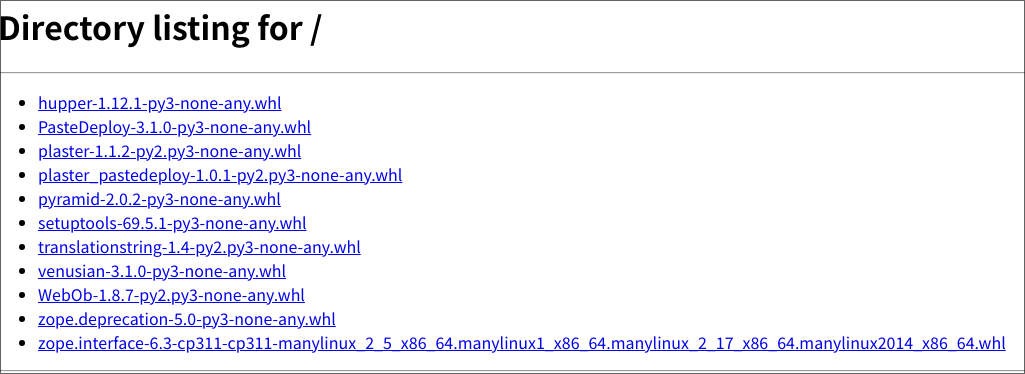
\includegraphics[width=.9\linewidth]{./http-server-simple-repository.png}
\end{center}
\end{frame}

\begin{frame}[label={sec:org268a1b8},fragile]{URL指定でインストール}
 \begin{itemize}
\item pipはURL指定で直接インストールできる
\item 正確なファイル名を知らないといけない
\item wheelはプラットフォームなどの情報を含んでいる
\end{itemize}

\begin{verbatim}
pip install \
    http://localhost:8000/pyramid-2.0.2-py3-none-any.whl
\end{verbatim}
\end{frame}

\begin{frame}[label={sec:orgb797a29},fragile]{複雑なwheelファイル名}
 \begin{itemize}
\item oh\ldots{}
\end{itemize}
\begin{verbatim}
zope.interface-6.4
-cp311
-cp311
-manylinux_2_5_x86_64.manylinux1_x86_64.manylinux_2_17_x86_64.manylinux2014_x86_64
.whl
\end{verbatim}
\end{frame}
\begin{frame}[label={sec:orgeadba72},fragile]{find-links}
 \begin{itemize}
\item \texttt{find-links} で指定した場所から探しだしてもらう
\end{itemize}
\begin{verbatim}
pip install -f http://localhost:8000 zope.interface
\end{verbatim}
\end{frame}

\begin{frame}[label={sec:orgf40c688},fragile]{no-index}
 \begin{itemize}
\item 場合によってはpypiへの接続も制限される環境
\item 全てをお手軽repositoryから取得するなら \texttt{no-index} も使うようにしてみよう

\item \texttt{no-index} pypiなどのindexを見にいかない
\item \texttt{find-url} 指定したページからダウンロードURLをスクレーピング
\end{itemize}
\end{frame}

\begin{frame}[label={sec:org92a6398},fragile]{indexは必要?}
 \begin{itemize}
\item pipを直接使うなら \texttt{find-url} でもいいかも?
\item メタデータを取得するのに配布物をダウンロードするという効率の悪さはある
\item \texttt{poetry source add} で使えるのは simple repository
\begin{itemize}
\item pipだと \texttt{-{}-{}index-url} で指定するものに相当
\end{itemize}
\end{itemize}
\end{frame}

\begin{frame}[label={sec:org80c3d8c},fragile]{独自のpypiを立てたい!}
 \begin{itemize}
\item PyPI自体のソースコードは公開されている
\begin{itemize}
\item \url{https://github.com/pypi/warehouse}
\item インフラ構築保守など手間もかかる
\end{itemize}
\item devpi
\begin{itemize}
\item \url{https://github.com/devpi/devpi}
\item PyPIへのプロキシやプロジェクトごとの名前空間設定など多機能
\item それなりにインフラ構築保守の手間がかかる
\end{itemize}
\item \texttt{http.server} くらいに簡単に立ち上って欲しいところ
\end{itemize}
\end{frame}

\section{パッケージを配るためのPEP}
\label{sec:org95d80cc}
\begin{frame}[label={sec:org49eac7c}]{パッケージを配るためのPEP}
\begin{itemize}
\item \href{https://peps.python.org/pep-0458}{PEP 458 – Secure PyPI downloads with signed repository metadata}
\item \href{https://peps.python.org/pep-0480}{PEP 480 – Surviving a Compromise of PyPI: End-to-end signing of packages}
\item \href{https://peps.python.org/pep-0503/}{PEP 503 – Simple Repository API}
\item \href{https://peps.python.org/pep-0592}{PEP 592 – Adding “Yank” Support to the Simple API}
\item \href{https://peps.python.org/pep-0629}{PEP 629 – Versioning PyPI’s Simple API}
\item \href{https://peps.python.org/pep-0658}{PEP 658 – Serve Distribution Metadata in the Simple Repository API}
\item \href{https://peps.python.org/pep-0691}{PEP 691 – JSON-based Simple API for Python Package Indexes}
\item \href{https://peps.python.org/pep-0700}{PEP 700 – Additional Fields for the Simple API for Package Indexes}
\item \href{https://peps.python.org/pep-0714}{PEP 714 – Rename dist-info-metadata in the Simple API}
\end{itemize}
\end{frame}

\begin{frame}[label={sec:orga1c4f19}]{Simple Repository}
representation

\begin{itemize}
\item HTML PEP503
\item JSON PEP691
\end{itemize}

バージョン
\begin{itemize}
\item 1.0 PEP503/PEP691
\item 1.1 PEP700
\item PEP714 メタデータフィールドの取り扱いについての修正
\begin{itemize}
\item warehouseの実装で間違えがあったらしい
\end{itemize}
\end{itemize}
\end{frame}

\begin{frame}[label={sec:org885d0b3}]{PyPIのSimple Repository}
\begin{itemize}
\item \url{https://pypi.org/simple/} とても大きいのでアクセス注意!
\end{itemize}
\end{frame}


\begin{frame}[label={sec:org0bab675}]{実装方針}
\begin{itemize}
\item 標準ライブラリでいこう
\begin{itemize}
\item Batteries Included!
\end{itemize}
\item 1ファイルデプロイ
\item DBなどを使わず起動するだけで使える
\end{itemize}
\end{frame}

\begin{frame}[label={sec:org84d9f99}]{標準ライブラリでwebアプリケーションを書く}
\begin{itemize}
\item json
\item wsgiref
\end{itemize}
\end{frame}

\begin{frame}[label={sec:org8a443cd},fragile]{project list}
 \begin{itemize}
\item ホストしているプロジェクト(ほぼパッケージの意味)を一覧で出すだけ
\item v1.0のプロジェクトに関する情報は \texttt{name} のみ
\end{itemize}
\end{frame}

\begin{frame}[label={sec:orgaffa90a},fragile]{使うライブラリ}
 \begin{itemize}
\item これだけ!
\item 100\% 標準ライブラリのみ!
\end{itemize}

\begin{verbatim}
import argparse
import hashlib
import itertools
import json
import operator
import pathlib
import re
import zipfile
from typing import TypedDict, NotRequired, Iterable
from wsgiref.types import WSGIApplication, WSGIEnvironment, StartResponse
from wsgiref.simple_server import make_server
\end{verbatim}
\end{frame}

\begin{frame}[label={sec:org7b8bbfe},fragile]{Meta}
 \begin{itemize}
\item simple repositoryに関する情報
\item バージョン
\end{itemize}

\begin{verbatim}
Meta = TypedDict(
    "Meta",
    {
        "api-version": str,
    },
)
\end{verbatim}
\end{frame}

\begin{frame}[label={sec:org12b3887}]{project detail}
\begin{itemize}
\item プロジェクト(パッケージ)ごとのダウンロード可能なファイル一覧
\item ファイルのURLやパッケージメタデータなど
\end{itemize}
\end{frame}

\begin{frame}[label={sec:org90ec309},fragile]{project fileのtyping}
 \begin{itemize}
\item 事前に確認可能なパッケージメタデータ
\item ダウンロードに必要な情報 URLやハッシュ
\end{itemize}

\begin{verbatim}
ProjectFile = TypedDict(
    "ProjectFile",
    {
        "filename": str,
        "url": str,
        "hashes": dict[str, str],
        "requires-python": NotRequired[str],
        "dist-info-metadata": NotRequired[str],
        "gpg-sig": NotRequired[bool],
        "yanked": NotRequired[bool],
    },
)

\end{verbatim}
\end{frame}

\begin{frame}[label={sec:orgb2f84d6},fragile]{project detailのtyping}
 \begin{itemize}
\item project fileの一覧が主な情報
\end{itemize}

\begin{verbatim}
ProjectDetail = TypedDict(
    "ProjectDetail",
    {
        "name": str,
        "files": list[ProjectFile],
        "meta": Meta,
    },
)

\end{verbatim}
\end{frame}

\begin{frame}[label={sec:org1889fc0},fragile]{project list のtyping}
 \begin{verbatim}
Project = TypedDict("Project", {"name": str})
ProjectList = TypedDict(
    "ProjectList",
    {
        "meta": Meta,
        "projects": list[Project],
    },
)

\end{verbatim}
\end{frame}

\begin{frame}[label={sec:orge26cead},fragile]{wheelファイルを探しだす}
 \begin{itemize}
\item pathlibでできちゃうね!
\end{itemize}

\begin{verbatim}
wheelhouse.glob("*.whl")
\end{verbatim}
\end{frame}

\begin{frame}[label={sec:org01ca322},fragile]{wheelファイル名から情報を取得}
 \begin{itemize}
\item wheelファイルのファイル名は形式が決まっている
\begin{itemize}
\item PEP 491 The Wheel Binary Package Format 1.9
\item \texttt{\{distribution\}-\{version\}(-\{build tag\})?-\{python tag\}-\{abi tag\}-\{platform tag\}.whl.}
\end{itemize}
\end{itemize}
\end{frame}

\begin{frame}[label={sec:org0cedec8},fragile]{wheelファイル名から情報を取得}
 \begin{itemize}
\item 今回欲しいのは \texttt{distiribution}
\item \texttt{"-"} で \texttt{split} して最初の1つ
\end{itemize}

\begin{verbatim}
def extract_dist_name(wh: pathlib.Path) -> str:
    return wh.name.split("-", 1)[0]
\end{verbatim}
\end{frame}

\begin{frame}[label={sec:org56871a4},fragile]{プロジェクト名を正規化}
 \begin{itemize}
\item PEP 503 で正式に正規化方法が定義されている
\item アルファベットは全て小文字
\item 記号は \texttt{-} に正規化
\item 例: \texttt{zope.interface} -> \texttt{zope-interface}
\end{itemize}

\begin{verbatim}
def normalize(name: str) -> str:
    return re.sub(r"[-_.]+", "-", name).lower()
\end{verbatim}
\end{frame}

\begin{frame}[label={sec:org3db9344},fragile]{metadata}
 \begin{itemize}
\item METADATAをwheelから取り出す
\item wheelはzipファイル
\item METADATAの場所は決まっている
\begin{itemize}
\item PEP 491 The Wheel Binary Package Format 1.9
\item \texttt{\{distribution\}-\{version\}.dist-info/} contains metadata.
\end{itemize}
\end{itemize}

\begin{verbatim}
def get_metadata(whl: pathlib.Path):
    parts = whl.name.split("-")
    dist_name, version = parts[0], parts[1]
    metadata_path = f"{dist_name}-{version}.dist-info/METADATA"
    with zipfile.ZipFile(whl) as zf:
        with zf.open(metadata_path) as metadata:
            return metadata.read()

\end{verbatim}
\end{frame}

\begin{frame}[label={sec:orge6c21bb},fragile]{全部まとめてwheelファイルの情報を取得}
 \begin{itemize}
\item プロジェクト名をキーにしてメタデータとwheelファイルパスをグルーピング
\end{itemize}

\begin{verbatim}
def load_wheels(
    wheelhouse: pathlib.Path,
) -> itertools.groupby[str, tuple[str, bytes, pathlib.Path]]:
    wheels = itertools.groupby(
        (
            (normalize(extract_dist_name(w)), get_metadata(w), w)
            for w in wheelhouse.glob("*.whl")
        ),
        key=operator.itemgetter(0),
    )
    return wheels
\end{verbatim}
\end{frame}
\begin{frame}[label={sec:org39795ed},fragile]{プロジェクトごとにファイル情報をまとめる}
 \begin{itemize}
\item プロジェクト名、メタデータ、wheelファイルパスをもとにJSONデータを作成
\end{itemize}

\begin{verbatim}
def load_projects(
    wheelhouse: pathlib.Path,
) -> tuple[ProjectList, dict[str, ProjectDetail]]:
    meta = Meta({"api-version": "1.0"})

    project_list = ProjectList(
        {
            "meta": meta,
            "projects": [],
        }
    )

    project_details: dict[str, ProjectDetail] = {}
    for project_name, files in load_wheels(wheelhouse):
        project = ProjectDetail({"name": project_name, "files": [], "meta": meta})
        project_list["projects"].append(Project({"name": project_name}))
        project_details[project_name] = project
        for _, metadata, p in files:
            f = ProjectFile(
                {
                    "filename": p.name,
                    "url": f"{project_name}/files/{p.name}",
                    "hashes": {
                        "sha256": hashlib.sha256(p.read_bytes()).hexdigest(),
                    },
                    "dist-info-metadata": metadata.decode("utf-8"),
                }
            )
            project["files"].append(f)
    return project_list, project_details

\end{verbatim}
\end{frame}

\begin{frame}[label={sec:org89eba0c},fragile]{wsgiアプリケーション:project list}
 \begin{verbatim}
class ProjectListApp:
    def __init__(self, project_list: ProjectList) -> None:
        self.project_list = project_list

    def __call__(
        self, environ: WSGIEnvironment, start_response: StartResponse
    ) -> Iterable[bytes]:
        start_response(
            "200 OK", [("Content-Type", "application/vnd.pypi.simple.v1+json")]
        )
        return [json.dumps(self.project_list).encode("utf-8")]

\end{verbatim}
\end{frame}
\begin{frame}[label={sec:orga1814fe},fragile]{wsgiアプリケーション:project detail}
 \begin{verbatim}
class ProjectDetailApp:
    def __init__(self, project_details: dict[str, ProjectDetail]) -> None:
        self.project_details = project_details

    def __call__(
        self, environ: WSGIEnvironment, start_response: StartResponse
    ) -> Iterable[bytes]:
        project_name = environ["wsgiorg.routing_args"][1]["project_name"]
        if project_name not in self.project_details:
            start_response(
                "404 Not Found",
                [("Content-Type", "application/vnd.pypi.simple.v1+json")],
            )
            return [b""]
        start_response(
            "200 OK", [("Content-Type", "application/vnd.pypi.simple.v1+json")]
        )
        return [json.dumps(self.project_details[project_name]).encode("utf-8")]

\end{verbatim}
\end{frame}
\begin{frame}[label={sec:org6a32ac7},fragile]{wsgiアプリケーション:ダウンロード}
 \begin{itemize}
\item wheelファイルの中身をレスポンスボディにする
\item wheelのcontent-typeは特に決まってないので \texttt{application/octet-stream} にする
\item ブラウザでアクセスしたときにダウンロードになるよう \texttt{Content-Disposition} をつける
\end{itemize}

\begin{verbatim}
class WheelDownloadApp:
    def __init__(self, wheelhouse: pathlib.Path) -> None:
        self.wheelhouse = wheelhouse

    def __call__(
        self, environ: WSGIEnvironment, start_response: StartResponse
    ) -> Iterable[bytes]:
        file_name: str = environ["wsgiorg.routing_args"][1]["wheel_file_name"]
        p = self.wheelhouse / file_name
        if not p.exists():
            start_response(
                "404 Not Found",
                [("Content-Type", "application/vnd.pypi.simple.v1+json")],
            )
            return [b""]
        start_response(
            "200 OK",
            [
                ("Content-Type", "application/octed-stream"),
                ("Content-Disposition", f'attachment; filename="{file_name}"'),
            ],
        )
        with p.open("rb") as f:
            return f

\end{verbatim}
\end{frame}

\begin{frame}[label={sec:org8cad2b8},fragile]{WSGIアプリケーションのルーティング}
 \begin{itemize}
\item wsgi.orgのドキュメントにルーティングのサンプルがあるので流用
\item \url{https://wsgi.readthedocs.io/en/latest/specifications/routing\_args.html}
\end{itemize}
\begin{verbatim}
class RegexDispatch(object):
    def __init__(self, patterns: list[tuple[re.Pattern, WSGIApplication]]):
        self.patterns = patterns

    def __call__(
        self, environ: WSGIEnvironment, start_response: StartResponse
    ) -> Iterable[bytes]:
        script_name: str = environ.get("SCRIPT_NAME", "")
        path_info: str = environ.get("PATH_INFO", "")
        for regex, application in self.patterns:
            match = regex.match(path_info)
            if not match:
                continue
            extra_path_info = path_info[match.end() :]
            if extra_path_info and not extra_path_info.startswith("/"):
                # Not a very good match
                continue
            pos_args = match.groups()
            named_args = match.groupdict()
            cur_pos, cur_named = environ.get("wsgiorg.routing_args", ((), {}))
            new_pos = list(cur_pos) + list(pos_args)
            new_named = cur_named.copy()
            new_named.update(named_args)
            environ["wsgiorg.routing_args"] = (new_pos, new_named)
            environ["SCRIPT_NAME"] = script_name + path_info[: match.end()]
            environ["PATH_INFO"] = extra_path_info
            return application(environ, start_response)
        return self.not_found(environ, start_response)

    def not_found(self, environ, start_response) -> Iterable[bytes]:
        start_response("404 Not Found", [("Content-type", "text/plain")])
        return [b"Not found"]

\end{verbatim}
\end{frame}

\begin{frame}[label={sec:orgab7a573},fragile]{simple repositoryの機能}
 \begin{itemize}
\item \texttt{/} project list
\item \texttt{/\{project\}} project detail
\item 実際にwheelファイルをダウンロードするURL
\begin{itemize}
\item 今回は \texttt{/\{project\}/files/\{wheel\}} にします
\end{itemize}
\end{itemize}

\begin{verbatim}
def make_app(wheelhouse: pathlib.Path) -> WSGIApplication:
    (project_list, project_details) = load_projects(wheelhouse)
    app: WSGIApplication = RegexDispatch(
        [
            (re.compile(r"^/$"), ProjectListApp(project_list)),
            (
                re.compile(r"^/(?P<project_name>\w+)$"),
                ProjectDetailApp(project_details),
            ),
            (
                re.compile(
                    r"^/(?P<project_name>\w+)/files/(?P<wheel_file_name>\w\.whl)$"
                ),
                ProjectDetailApp(project_details),
            ),
        ]
    )
    return app
\end{verbatim}
\end{frame}

\begin{frame}[label={sec:orgb67fb32},fragile]{さあ!wsgiアプリケーションを立ち上げよう!}
 \begin{itemize}
\item 重要なのはwheelファイルを置いてある \texttt{wheelhouse} ディレクトリ
\item \texttt{host}, \texttt{port} はwebアプリケーションとして必要な情報
\end{itemize}

\begin{verbatim}
def main() -> None:
    parser = argparse.ArgumentParser()
    parser.add_argument("wheelhouse", type=pathlib.Path)
    parser.add_argument("--host", type=str, default="0.0.0.0")
    parser.add_argument("--port", type=int, default=8000)
    args = parser.parse_args()
    app = make_app(args.wheelhouse)
    httpd = make_server(args.host, args.port, app)
    httpd.serve_forever()


if __name__ == "__main__":
    main()
\end{verbatim}
\end{frame}

\begin{frame}[label={sec:orgef1b595},fragile]{pipから使う}
 \begin{itemize}
\item project list呼ばれてないかも?
\end{itemize}


\begin{verbatim}
$ pip install pyramid --index-url=http://localhost:8000/
\end{verbatim}
\end{frame}

\begin{frame}[label={sec:org5c7697c}]{The Update Framework}
\begin{itemize}
\item TUF
\end{itemize}
\end{frame}

\section{参考文献}
\label{sec:org138cf77}
\begin{frame}[label={sec:org1ac519d}]{参考文献}
\begin{itemize}
\item PyPA Simple Repository API, \url{https://packaging.python.org/en/latest/specifications/simple-repository-api/}
\item The Update Framework, \url{https://theupdateframework.io/}
\end{itemize}
\end{frame}
\end{document}
